\documentclass[12pt]{article}
\usepackage{hyperref,amsmath,amsfonts,amssymb,fullpage,color}
\usepackage{enumitem}
\usepackage{tikz}
\usetikzlibrary{arrows.meta,decorations.pathmorphing,calc,patterns}

\newcommand{\be}{\begin{equation}}
\newcommand{\ee}{\end{equation}}
\newcommand{\bh}{\bar{h}}

\newcounter{quesno}
\newcommand{\ques}[1]{\vspace{2.5em}\stepcounter{quesno}
\noindent{\bf\large Question \thequesno.} \emph{(#1 points)}\par\vspace{0.5em}
}

\begin{document}

\begin{center}
{\bf\Large General Relativity}

\vspace{0.8em}
{\bf\large Final Examination --- Model Solutions}
\end{center}

\vspace{0.5em}
\hrule
\vspace{0.5em}

%==============================================================================
% QUESTION 1
%==============================================================================
\ques{2}
\noindent
\textbf{Transformation of the Riemann tensor:}

Let $x^\mu$ and $x^{\mu'}$ be two coordinate systems related by a smooth, invertible coordinate transformation $x^\mu \mapsto x^{\mu'}(x)$. The Riemann curvature tensor $R^\mu{}_{\nu\rho\sigma}$ is a tensor of type $(1,3)$ (one contravariant index and three covariant indices). Under a change of coordinates $x^\mu \mapsto x^{\mu'}$, its components transform according to the tensor transformation law:
\be
R^{\mu'}{}_{\nu'\rho'\sigma'}(x') = \frac{\partial x^{\mu'}}{\partial x^\mu} \frac{\partial x^\nu}{\partial x^{\nu'}} \frac{\partial x^\rho}{\partial x^{\rho'}} \frac{\partial x^\sigma}{\partial x^{\sigma'}} R^\mu{}_{\nu\rho\sigma}(x) \,.
\label{eq:riemann_trans}
\ee

\medskip
\noindent
\textbf{Transformation of the Ricci tensor:}

The Ricci tensor is defined in any coordinate system by contracting the first (contravariant) index with the third (covariant) index of the Riemann tensor:
\be
R_{\mu\nu} = R^\rho{}_{\mu\rho\nu} \,.
\ee
In the primed coordinate system $x^{\mu'}$, the components of the Ricci tensor are therefore given by $R_{\mu'\nu'} = R^{\rho'}{}_{\mu'\rho'\nu'}$. Setting $\mu' = \rho'$ in equation~\eqref{eq:riemann_trans} and summing over the repeated index $\rho'$ (with dummy indices relabelled appropriately to avoid confusion), we obtain:
\be
R_{\mu'\nu'}(x') = R^{\rho'}{}_{\mu'\rho'\nu'}(x') = \frac{\partial x^{\rho'}}{\partial x^\alpha} \frac{\partial x^\mu}{\partial x^{\mu'}} \frac{\partial x^\beta}{\partial x^{\rho'}} \frac{\partial x^\nu}{\partial x^{\nu'}} R^\alpha{}_{\mu\beta\nu}(x) \,.
\ee
By the multivariable chain rule, the Jacobian matrices $\frac{\partial x^{\rho'}}{\partial x^\alpha}$ and $\frac{\partial x^\beta}{\partial x^{\rho'}}$ are inverses of one another:
\be
\frac{\partial x^{\rho'}}{\partial x^\alpha} \frac{\partial x^\beta}{\partial x^{\rho'}} = \frac{\partial x^\beta}{\partial x^\alpha} = \delta^\beta_\alpha \,,
\ee
where $\delta^\beta_\alpha$ is the Kronecker delta. Substituting this identity into the expression for $R_{\mu'\nu'}(x')$ yields:
\begin{align}
R_{\mu'\nu'}(x') &= \delta^\beta_\alpha \frac{\partial x^\mu}{\partial x^{\mu'}} \frac{\partial x^\nu}{\partial x^{\nu'}} R^\alpha{}_{\mu\beta\nu}(x) \nonumber \\
&= \frac{\partial x^\mu}{\partial x^{\mu'}} \frac{\partial x^\nu}{\partial x^{\nu'}} R^\alpha{}_{\mu\alpha\nu}(x) \nonumber \\
&= \frac{\partial x^\mu}{\partial x^{\mu'}} \frac{\partial x^\nu}{\partial x^{\nu'}} R_{\mu\nu}(x) \,.
\end{align}
This is precisely the transformation law for the components of a $(0,2)$ tensor under a change of coordinates. Hence $R_{\mu\nu}$ transforms as a rank $(0,2)$ tensor.


%==============================================================================
% QUESTION 2
%==============================================================================
\ques{3}
We are given a manifold equipped with a metric $g_{\mu\nu}$ and a totally antisymmetric $(0,3)$ tensor $H_{\mu\nu\rho} = H_{[\mu\nu\rho]}$, along with the connection
\be
\hat \Gamma_{\mu\nu}{}^\rho = \Gamma_{\mu\nu}{}^\rho + \frac{1}{12} g^{\rho \sigma} H_{\mu\nu\sigma} \,,
\label{eq:stringconn_ans}
\ee
where $\Gamma_{\mu\nu}{}^\rho$ are the components of the Levi-Civita connection.

\begin{enumerate}[label=\alph*)]
\item \textbf{Torsion and metric compatibility:}

\emph{1. Is $\hat\Gamma_{\mu\nu}{}^\rho$ torsion-free?}

The torsion tensor $\hat{T}_{\mu\nu}{}^\rho$ of a connection $\hat\Gamma_{\mu\nu}{}^\rho$ is defined as twice the antisymmetric part of the connection coefficients in their lower indices:
\be
\hat{T}_{\mu\nu}{}^\rho = 2 \hat\Gamma_{[\mu\nu]}{}^\rho = \hat\Gamma_{\mu\nu}{}^\rho - \hat\Gamma_{\nu\mu}{}^\rho \,.
\ee
Substituting equation~\eqref{eq:stringconn_ans}:
\be
\hat{T}_{\mu\nu}{}^\rho = \left( \Gamma_{\mu\nu}{}^\rho - \Gamma_{\nu\mu}{}^\rho \right) + \frac{1}{12} g^{\rho\sigma} \left( H_{\mu\nu\sigma} - H_{\nu\mu\sigma} \right) \,.
\ee
Since the Levi-Civita connection $\Gamma_{\mu\nu}{}^\rho$ is torsion-free, it is symmetric in its lower indices, $\Gamma_{\mu\nu}{}^\rho = \Gamma_{\nu\mu}{}^\rho$, so the first term vanishes. Since $H_{\mu\nu\sigma}$ is totally antisymmetric, it satisfies $H_{\nu\mu\sigma} = -H_{\mu\nu\sigma}$. Therefore:
\be
\hat{T}_{\mu\nu}{}^\rho = \frac{1}{6} g^{\rho\sigma} H_{\mu\nu\sigma} = \frac{1}{6} H_{\mu\nu}{}^\rho \neq 0 \quad (\text{for non-zero } H_{\mu\nu\rho}) \,.
\ee
Thus, the connection $\hat\Gamma_{\mu\nu}{}^\rho$ is \textbf{not torsion-free} (unless $H_{\mu\nu\rho} = 0$).

\medskip
\emph{2. Is $\hat\Gamma_{\mu\nu}{}^\rho$ metric compatible?}

A connection $\hat\nabla$ is metric compatible if and only if $\hat\nabla_\mu g_{\nu\rho} = 0$. Expanding the covariant derivative of the metric with respect to $\hat\Gamma_{\mu\nu}{}^\rho$:
\be
\hat\nabla_\mu g_{\nu\rho} = \partial_\mu g_{\nu\rho} - \hat\Gamma_{\mu\nu}{}^\lambda g_{\lambda\rho} - \hat\Gamma_{\mu\rho}{}^\lambda g_{\nu\lambda} \,.
\ee
Substituting the definition~\eqref{eq:stringconn_ans} of $\hat\Gamma_{\mu\nu}{}^\lambda$:
\begin{align}
\hat\nabla_\mu g_{\nu\rho} &= \partial_\mu g_{\nu\rho} - \left( \Gamma_{\mu\nu}{}^\lambda + \frac{1}{12} g^{\lambda\sigma} H_{\mu\nu\sigma} \right) g_{\lambda\rho} - \left( \Gamma_{\mu\rho}{}^\lambda + \frac{1}{12} g^{\lambda\sigma} H_{\mu\rho\sigma} \right) g_{\nu\lambda} \nonumber \\
&= \left( \partial_\mu g_{\nu\rho} - \Gamma_{\mu\nu}{}^\lambda g_{\lambda\rho} - \Gamma_{\mu\rho}{}^\lambda g_{\nu\lambda} \right) - \frac{1}{12} g^{\lambda\sigma} g_{\lambda\rho} H_{\mu\nu\sigma} - \frac{1}{12} g^{\lambda\sigma} g_{\nu\lambda} H_{\mu\rho\sigma} \nonumber \\
&= \nabla_\mu g_{\nu\rho} - \frac{1}{12} \delta^\sigma_\rho H_{\mu\nu\sigma} - \frac{1}{12} \delta^\sigma_\nu H_{\mu\rho\sigma} \nonumber \\
&= \nabla_\mu g_{\nu\rho} - \frac{1}{12} \left( H_{\mu\nu\rho} + H_{\mu\rho\nu} \right) \,.
\end{align}
Here $\nabla_\mu g_{\nu\rho} = 0$ because the Levi-Civita connection $\Gamma_{\mu\nu}{}^\lambda$ is metric compatible by definition. Moreover, because $H_{\mu\nu\rho}$ is totally antisymmetric, it is antisymmetric in its last two indices: $H_{\mu\rho\nu} = -H_{\mu\nu\rho}$, which implies $H_{\mu\nu\rho} + H_{\mu\rho\nu} = 0$. Hence:
\be
\hat\nabla_\mu g_{\nu\rho} = 0 \,.
\ee
Therefore, the connection $\hat\Gamma_{\mu\nu}{}^\rho$ \textbf{is metric compatible}.

\item \textbf{Equivalence of geodesics:}

An affinely parametrised curve $x^\mu(\lambda)$ with tangent vector $\dot{x}^\mu = \frac{dx^\mu}{d\lambda}$ is a geodesic (autoparallel curve) of the connection $\hat\Gamma_{\mu\nu}{}^\rho$ if it satisfies the geodesic equation:
\be
\dot{x}^\mu \hat\nabla_\mu \dot{x}^\rho = \frac{d^2 x^\rho}{d\lambda^2} + \hat\Gamma_{\mu\nu}{}^\rho \frac{dx^\mu}{d\lambda} \frac{dx^\nu}{d\lambda} = 0 \,.
\ee
Substituting equation~\eqref{eq:stringconn_ans} into the geodesic equation gives:
\be
\frac{d^2 x^\rho}{d\lambda^2} + \Gamma_{\mu\nu}{}^\rho \frac{dx^\mu}{d\lambda} \frac{dx^\nu}{d\lambda} + \frac{1}{12} g^{\rho\sigma} H_{\mu\nu\sigma} \frac{dx^\mu}{d\lambda} \frac{dx^\nu}{d\lambda} = 0 \,.
\ee
In the third term, the product $\frac{dx^\mu}{d\lambda} \frac{dx^\nu}{d\lambda}$ is symmetric under the exchange of the dummy indices $\mu \leftrightarrow \nu$, whereas $H_{\mu\nu\sigma}$ is antisymmetric under $\mu \leftrightarrow \nu$ ($H_{\mu\nu\sigma} = -H_{\nu\mu\sigma}$). Contracting a symmetric tensor with an antisymmetric tensor yields zero identically:
\be
H_{\mu\nu\sigma} \frac{dx^\mu}{d\lambda} \frac{dx^\nu}{d\lambda} = \frac{1}{2} \left( H_{\mu\nu\sigma} + H_{\nu\mu\sigma} \right) \frac{dx^\mu}{d\lambda} \frac{dx^\nu}{d\lambda} = 0 \,.
\ee
Consequently, the $H_{\mu\nu\sigma}$ contribution drops out completely, and the geodesic equation for $\hat\Gamma_{\mu\nu}{}^\rho$ reduces to
\be
\frac{d^2 x^\rho}{d\lambda^2} + \Gamma_{\mu\nu}{}^\rho \frac{dx^\mu}{d\lambda} \frac{dx^\nu}{d\lambda} = 0 \,,
\ee
which is the exact geodesic equation for the Levi-Civita connection $\Gamma_{\mu\nu}{}^\rho$. Thus, the geodesics of $\hat\Gamma_{\mu\nu}{}^\rho$ are identical to the geodesics of the Levi-Civita connection.
\end{enumerate}


%==============================================================================
% QUESTION 3
%==============================================================================
\ques{4}
The Schwarzschild metric is given by
\be
ds^2 = - f(r) dt^2 + f(r)^{-1} dr^2 + r^2 d \theta^2 + r^2 \sin^2 \theta d\phi^2 \,, \qquad f(r) = 1 - \frac{2GM}{r} \,.
\ee

\begin{enumerate}[label=\alph*)]
\item \textbf{Singularities in the Schwarzschild metric and physical interpretation:}

\emph{1. Locations of the singularities:}

Examining the metric components $g_{\mu\nu}$ and inverse metric components $g^{\mu\nu}$ in the Schwarzschild coordinates $(t,r,\theta,\phi)$, we see that pathologies occur at:
\begin{itemize}
\item $r = 2GM$ (the \textbf{Schwarzschild radius / event horizon}): here $f(r) = 0$, so $g_{tt} = 0$ and $g_{rr} = \left(1 - \frac{2GM}{r}\right)^{-1} \to \infty$ (while $g^{tt} \to -\infty$).
\item $r = 0$ (the \textbf{central singularity}): here $f(r) \to -\infty$, so $g_{tt} \to \infty$, $g^{rr} \to -\infty$, and the two-sphere metric components $g_{\theta\theta}, g_{\phi\phi} \to 0$.
\item ($\theta = 0, \pi$: here $g_{\phi\phi} = r^2\sin^2\theta = 0$ and $g^{\phi\phi} \to \infty$, which is simply the standard coordinate singularity of spherical polar coordinates on $S^2$.)
\end{itemize}

\emph{2. Distinguishing coordinate vs.\ physical singularities:}

Because metric components depend on the choice of coordinates, a divergence in $g_{\mu\nu}$ or $g^{\mu\nu}$ does not necessarily mean spacetime itself is singular. To test whether a singularity is a true physical (curvature) singularity or merely an artifact of bad coordinates, we examine coordinate-independent scalar invariants built from the Riemann tensor. Since the Schwarzschild metric is a vacuum solution ($R_{\mu\nu} = 0$ and $R = 0$), the relevant non-vanishing curvature invariant is the \textbf{Kretschmann scalar}:
\be
K = R^{\mu\nu\rho\sigma} R_{\mu\nu\rho\sigma} = \frac{48 G^2 M^2}{r^6} \,.
\ee
\begin{itemize}
\item \textbf{At $r = 2GM$:} The Kretschmann scalar (along with all other curvature invariants) is completely finite:
\be
\left. R^{\mu\nu\rho\sigma} R_{\mu\nu\rho\sigma} \right|_{r = 2GM} = \frac{48 G^2 M^2}{(2GM)^6} = \frac{3}{4 (GM)^4} < \infty \,.
\ee
Therefore, $r = 2GM$ is only a \textbf{coordinate singularity}, resulting from the breakdown of the Schwarzschild coordinates $(t,r)$ at the horizon. Locally, the spacetime geometry is completely smooth at $r = 2GM$, and for a sufficiently supermassive black hole ($M$ large), the tidal forces at $r = 2GM$ are small enough that you can fall across $r = 2GM$ without feeling anything unusual at that moment.

\item \textbf{At $r = 0$:} The Kretschmann scalar diverges:
\be
\lim_{r \to 0} R^{\mu\nu\rho\sigma} R_{\mu\nu\rho\sigma} = \lim_{r \to 0} \frac{48 G^2 M^2}{r^6} = \infty \,.
\ee
Because a scalar takes the same value in every coordinate system, this divergence cannot be removed by any coordinate transformation. Thus, $r = 0$ is a \textbf{true physical (curvature) singularity}.
\end{itemize}

\emph{3. Which should you be genuinely concerned about, and why?}
\begin{itemize}
\item You must be genuinely concerned about the \textbf{physical curvature singularity at $r = 0$}, because as $r \to 0$ the spacetime curvature and gravitational tidal forces diverge to infinity, stretching you radially and compressing you transversely (``spaghettification'') until you are destroyed.
\item Furthermore, even though $r = 2GM$ is not a curvature singularity, you should \textbf{also} be concerned about crossing $r = 2GM$ because it is an \textbf{event horizon} (a causal boundary of no return). Once you cross into the interior region $r < 2GM$, the coordinate $r$ becomes timelike ($g_{rr} < 0$) and all future-directed timelike and null worldlines are forced toward decreasing $r$. You can never escape back to $r > 2GM$ or send any signal to your friends and family, and you are inevitably doomed to hit the lethal curvature singularity at $r = 0$ in a finite proper time ($\Delta \tau \le \pi GM$).
\end{itemize}

\item \textbf{Schwarzschild metric in ingoing Eddington-Finkelstein coordinates:}

We are given the ingoing Eddington-Finkelstein coordinate
\be
v = t + r + 2GM \ln\left| \frac{r}{2GM} - 1 \right| \,.
\ee
Taking the differential $dv$ (valid for both $r > 2GM$ and $r < 2GM$ since $\frac{d}{dx}\ln|x| = \frac{1}{x}$):
\begin{align}
dv &= dt + \left( 1 + \frac{2GM}{\frac{r}{2GM} - 1} \cdot \frac{1}{2GM} \right) dr \nonumber \\
&= dt + \left( 1 + \frac{2GM}{r - 2GM} \right) dr \nonumber \\
&= dt + \left( \frac{r}{r - 2GM} \right) dr \nonumber \\
&= dt + \left( 1 - \frac{2GM}{r} \right)^{-1} dr = dt + f(r)^{-1} dr \,.
\end{align}
Rearranging for $dt$ and squaring gives:
\begin{align}
dt &= dv - f(r)^{-1} dr \,, \\
dt^2 &= dv^2 - 2 f(r)^{-1} dv\, dr + f(r)^{-2} dr^2 \,.
\end{align}
Substituting $dt^2$ into the Schwarzschild line element:
\begin{align}
ds^2 &= -f(r) \left( dv^2 - 2 f(r)^{-1} dv\, dr + f(r)^{-2} dr^2 \right) + f(r)^{-1} dr^2 + r^2 d\theta^2 + r^2 \sin^2\theta d\phi^2 \nonumber \\
&= -f(r) dv^2 + 2 dv\, dr - f(r)^{-1} dr^2 + f(r)^{-1} dr^2 + r^2 d\theta^2 + r^2 \sin^2\theta d\phi^2 \nonumber \\
&= -f(r) dv^2 + 2 dv\, dr + r^2 d\theta^2 + r^2 \sin^2\theta d\phi^2 \,.
\end{align}
Writing out $f(r) = 1 - \frac{2GM}{r}$ explicitly, the metric in ingoing Eddington-Finkelstein coordinates $(v,r,\theta,\phi)$ is:
\be
\boxed{ds^2 = -\left( 1 - \frac{2GM}{r} \right) dv^2 + 2 dv\, dr + r^2 d\theta^2 + r^2 \sin^2\theta d\phi^2 \,.}
\label{eq:ef_metric}
\ee

\medskip
\emph{How this supports the answer to part a):}
\begin{enumerate}[label=\roman*.]
\item \textbf{Removal of the singularity at $r = 2GM$:} The singular $f(r)^{-1} dr^2$ term has cancelled identically against the cross-term from $dt^2$. At $r = 2GM$, $f(2GM) = 0$, and the metric~\eqref{eq:ef_metric} smoothly reduces to $ds^2 = 2 dv\, dr + (2GM)^2(d\theta^2 + \sin^2\theta d\phi^2)$, which has completely finite, regular components. Moreover, the metric is invertible at $r = 2GM$ because $\det(g_{\mu\nu}) = -r^4\sin^2\theta \neq 0$ (the $(v,r)$ block $\begin{pmatrix} -f(r) & 1 \\ 1 & 0 \end{pmatrix}$ has determinant $-1$ everywhere). This explicitly demonstrates that the singularity at $r = 2GM$ in Schwarzschild coordinates was merely a \textbf{coordinate singularity}, and that an infalling observer crosses $r = 2GM$ smoothly along a regular worldline (e.g.\ at finite $v$).
\item \textbf{Persistence of the physical singularity at $r = 0$:} In contrast, at $r = 0$ the metric component $g_{vv} = -\left(1 - \frac{2GM}{r}\right)$ still blows up to $+\infty$, consistent with $r = 0$ being a genuine \textbf{physical curvature singularity} that cannot be removed by changing coordinates.
\item \textbf{Causal trapping inside the horizon ($r \le 2GM$):} Radial null rays ($d\theta = d\phi = 0$, $ds^2 = 0$) satisfy
\be
dv \left[ -\left( 1 - \frac{2GM}{r} \right) dv + 2 dr \right] = 0 \,,
\ee
giving $dv = 0$ (ingoing light rays) and $\frac{dr}{dv} = \frac{1}{2}\left(1 - \frac{2GM}{r}\right)$ (outgoing light rays). At $r = 2GM$, $\frac{dr}{dv} = 0$, so outgoing light is frozen at the horizon; for $r < 2GM$, $1 - \frac{2GM}{r} < 0$, so $\frac{dr}{dv} < 0$ for \emph{all} future-directed null and timelike curves ($ds^2 \le 0$ with $dv > 0$). Thus any observer who falls past $r = 2GM$ cannot escape and is forced into the singularity at $r = 0$.
\end{enumerate}
\end{enumerate}


%==============================================================================
% QUESTION 4
%==============================================================================
\ques{5}
The de Sitter metric is
\be
ds^2 =- dt^2 +  L^2  \cosh^2 (t/L) \left( d\chi^2 + \sin^2 \chi \left( d\theta^2 + \sin^2\theta d\phi^2 \right)\right)  \,,
\label{eq:dsmetric_ans}
\ee
where $t \in (-\infty, \infty)$, $\chi \in (0,\pi)$, and $(\theta,\phi)$ are standard coordinates on $S^2$.

\begin{enumerate}[label=\alph*)]
\item \textbf{de Sitter as a candidate cosmological solution and the scale factor:}

\emph{Why it is a candidate cosmological solution for our universe:}
\begin{enumerate}[label=\roman*.]
\item \textbf{Homogeneity and Isotropy (Cosmological Principle):} On large scales ($\gtrsim 100\text{ Mpc}$), our universe is observed (via the Cosmic Microwave Background and large-scale galaxy surveys) to be spatially homogeneous and isotropic. In the metric~\eqref{eq:dsmetric_ans}, the spatial slices of constant cosmic time $t$ are three-spheres $S^3$ with round metric $d\Omega_3^2 = d\chi^2 + \sin^2\chi(d\theta^2 + \sin^2\theta d\phi^2)$. Because $S^3$ is a maximally symmetric 3-space (of constant positive curvature $k = +1$), the de Sitter metric is a special case of the \textbf{Friedmann-Lema\^{\i}tre-Robertson-Walker (FLRW)} metric:
\be
ds^2 = -dt^2 + a(t)^2 \left( d\chi^2 + \sin^2\chi \left( d\theta^2 + \sin^2\theta d\phi^2 \right) \right) \,.
\ee
\item \textbf{Accelerated Expansion and Dark Energy / Inflation:} The de Sitter metric solves Einstein's equations $G_{\mu\nu} + \Lambda g_{\mu\nu} = 0$ with a positive cosmological constant $\Lambda = \frac{3}{L^2} > 0$ (vacuum energy). For $t > 0$, the spatial sections expand ($\dot{a} > 0$) at an accelerating rate ($\ddot{a} = \frac{a}{L^2} > 0$), growing exponentially as $a(t) \approx \frac{L}{2} e^{t/L}$ for $t \gg L$. This describes two crucial eras of our physical universe: the early-universe epoch of \textbf{cosmic inflation}, and the present/future \textbf{dark-energy-dominated era} in which our universe's expansion is accelerating and asymptotically approaching de Sitter space.
\end{enumerate}

\emph{Scale factor:}

Comparing the metric~\eqref{eq:dsmetric_ans} directly with the FLRW line element $ds^2 = -dt^2 + a(t)^2 d\Omega_3^2$, the scale factor is:
\be
\boxed{a(t) = L \cosh\left(\frac{t}{L}\right)}
\ee
(or $a(t) = \cosh(t/L)$ if the curvature radius $L$ is absorbed into the spatial metric on $S^3$).

\item \textbf{Why conformally related metrics $g_{\mu\nu} = \Omega^2 \bar{g}_{\mu\nu}$ share the same causal structure:}

The causal structure of a spacetime is defined by the light cones at every point---that is, by the partitioning of tangent vectors $V^\mu$ (and smooth curves $x^\mu(\lambda)$ with tangent $V^\mu = \frac{dx^\mu}{d\lambda}$) into timelike, null (lightlike), and spacelike categories.

Suppose $g_{\mu\nu}(x) = \Omega^2(x) \bar{g}_{\mu\nu}(x)$, where $\Omega(x)$ is a smooth, strictly non-vanishing function, so that $\Omega^2(x) > 0$ everywhere. For any tangent vector $V^\mu$, its norm squared in the two metrics is related by:
\be
g_{\mu\nu} V^\mu V^\nu = \Omega^2 \bar{g}_{\mu\nu} V^\mu V^\nu \qquad \left(\text{equivalently, } ds^2 = \Omega^2 d\bar{s}^2\right) \,.
\ee
Because $\Omega^2 > 0$ is strictly positive, multiplication by $\Omega^2$ preserves the sign (and zeros) of the quadratic form at every point:
\begin{itemize}
\item \textbf{Timelike:} $g_{\mu\nu} V^\mu V^\nu < 0 \iff \bar{g}_{\mu\nu} V^\mu V^\nu < 0$,
\item \textbf{Null (lightlike):} $g_{\mu\nu} V^\mu V^\nu = 0 \iff \bar{g}_{\mu\nu} V^\mu V^\nu = 0$,
\item \textbf{Spacelike:} $g_{\mu\nu} V^\mu V^\nu > 0 \iff \bar{g}_{\mu\nu} V^\mu V^\nu > 0$.
\end{itemize}
Thus, the light cones (and hence all timelike, null, and spacelike curves, as well as causal future/past relations between events) of $g_{\mu\nu}$ and $\bar{g}_{\mu\nu}$ are identical. Consequently, $g_{\mu\nu}$ and $\bar{g}_{\mu\nu}$ have the exact same causal structure.

\item \textbf{Conformal coordinate transformation and Penrose diagram of de Sitter space:}

We perform the coordinate transformation from cosmic time $t \in (-\infty, \infty)$ to conformal time $\eta$:
\be
\cosh \frac{t}{L} = \frac{1}{\cos \eta} \,.
\label{eq:eta_def}
\ee
Since $\cosh(t/L) \in [1, \infty)$ for $t \in (-\infty, \infty)$, the conformal time $\eta$ takes values in the finite open interval
\be
\eta \in \left( -\frac{\pi}{2}, \frac{\pi}{2} \right) \,,
\ee
with $t \to -\infty \implies \eta \to -\frac{\pi}{2}$, $t = 0 \implies \eta = 0$, and $t \to +\infty \implies \eta \to +\frac{\pi}{2}$.

Differentiating both sides of equation~\eqref{eq:eta_def} gives:
\be
\frac{1}{L} \sinh\left(\frac{t}{L}\right) dt = \frac{\sin\eta}{\cos^2\eta} d\eta \,.
\ee
Using the hyperbolic and trigonometric identities $\sinh^2(t/L) = \cosh^2(t/L) - 1 = \frac{1}{\cos^2\eta} - 1 = \frac{\sin^2\eta}{\cos^2\eta} = \tan^2\eta$ (with $\operatorname{sgn}(t) = \operatorname{sgn}(\eta)$, so $\sinh(t/L) = \frac{\sin\eta}{\cos\eta}$), we obtain:
\be
\frac{1}{L} \frac{\sin\eta}{\cos\eta} dt = \frac{\sin\eta}{\cos^2\eta} d\eta \quad \implies \quad dt = \frac{L}{\cos\eta} d\eta \,.
\ee
Substituting $dt = \frac{L}{\cos\eta} d\eta$ and $\cosh(t/L) = \frac{1}{\cos\eta}$ into the de Sitter metric~\eqref{eq:dsmetric_ans} yields:
\begin{align}
ds^2 &= -\frac{L^2}{\cos^2\eta} d\eta^2 + \frac{L^2}{\cos^2\eta} \left( d\chi^2 + \sin^2\chi \left( d\theta^2 + \sin^2\theta d\phi^2 \right) \right) \nonumber \\
&= \frac{L^2}{\cos^2\eta} \left[ -d\eta^2 + d\chi^2 + \sin^2\chi \left( d\theta^2 + \sin^2\theta d\phi^2 \right) \right] \,.
\end{align}
This is of the form $g_{\mu\nu} = \Omega^2(\eta) \bar{g}_{\mu\nu}$ with conformal factor $\Omega(\eta) = \frac{L}{\cos\eta}$ and unphysical metric
\be
d\bar{s}^2 = -d\eta^2 + d\chi^2 + \sin^2\chi \left( d\theta^2 + \sin^2\theta d\phi^2 \right) \,, \qquad \eta \in \left(-\frac{\pi}{2}, \frac{\pi}{2}\right), \quad \chi \in [0, \pi] \,.
\ee
In these coordinates, radial null rays ($d\theta = d\phi = 0, d\bar{s}^2 = 0$) obey $d\eta = \pm d\chi$, which are straight lines at $\pm 45^\circ$ in the $(\chi, \eta)$ plane.

\medskip
\noindent
\textbf{Penrose Diagram of de Sitter Spacetime:}

\begin{center}
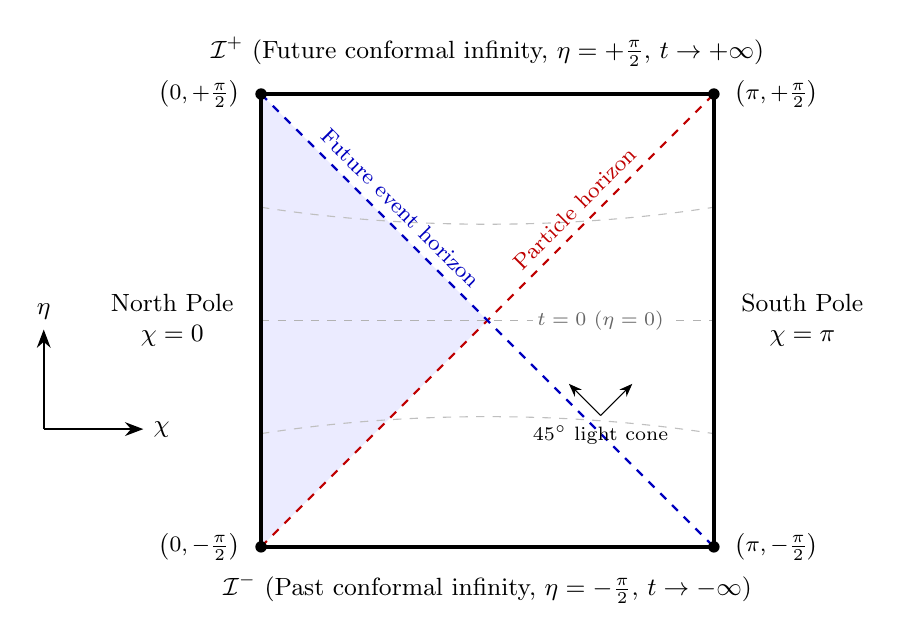
\begin{tikzpicture}[scale=1.15, >=Stealth]
    % Define coordinates for the square: chi in [0, 5], eta in [-2.5, 2.5]
    \coordinate (BL) at (0,-2.5);
    \coordinate (BR) at (5,-2.5);
    \coordinate (TL) at (0,2.5);
    \coordinate (TR) at (5,2.5);

    % Shaded causal diamond (static patch) for an observer at the North Pole chi=0
    \fill[blue!8] (0,-2.5) -- (2.5,0) -- (0,2.5) -- cycle;

    % Constant-t curves (spacelike hypersurfaces)
    \draw[gray!60, dashed, thin] (0, 0) -- (5, 0);
    \node[gray!80!black, font=\scriptsize, fill=white, inner sep=1.5pt] at (3.75, 0) {$t = 0\ (\eta = 0)$};
    \draw[gray!50, dashed, thin] (0, 1.25) .. controls (1.6, 1.0) and (3.4, 1.0) .. (5, 1.25);
    \draw[gray!50, dashed, thin] (0,-1.25) .. controls (1.6,-1.0) and (3.4,-1.0) .. (5,-1.25);

    % Cosmological horizons (diagonals at 45 degrees)
    \draw[red!75!black, thick, dashed] (0,-2.5) -- (5,2.5) node[pos=0.72, sloped, above, font=\footnotesize] {Particle horizon};
    \draw[blue!75!black, thick, dashed] (0,2.5) -- (5,-2.5) node[pos=0.28, sloped, above, font=\footnotesize] {Future event horizon};

    % Boundary of the Penrose diagram (square of side pi)
    % Left and right vertical lines: North and South poles of S^3
    \draw[very thick] (BL) -- (TL) node[midway, left=6pt, align=center, font=\small] {North Pole\\$\chi = 0$};
    \draw[very thick] (BR) -- (TR) node[midway, right=6pt, align=center, font=\small] {South Pole\\$\chi = \pi$};

    % Top and bottom horizontal lines: Spacelike conformal infinities
    \draw[very thick] (TL) -- (TR) node[midway, above=6pt, font=\small] {$\mathcal{I}^+$ (Future conformal infinity, $\eta = +\frac{\pi}{2},\, t \to +\infty$)};
    \draw[very thick] (BL) -- (BR) node[midway, below=6pt, font=\small] {$\mathcal{I}^-$ (Past conformal infinity, $\eta = -\frac{\pi}{2},\, t \to -\infty$)};

    % Corner labels placed cleanly to the left and right of the vertices
    \fill (BL) circle (1.8pt) node[left=4pt, font=\footnotesize] {$\left(0, -\frac{\pi}{2}\right)$};
    \fill (BR) circle (1.8pt) node[right=4pt, font=\footnotesize] {$\left(\pi, -\frac{\pi}{2}\right)$};
    \fill (TL) circle (1.8pt) node[left=4pt, font=\footnotesize] {$\left(0, +\frac{\pi}{2}\right)$};
    \fill (TR) circle (1.8pt) node[right=4pt, font=\footnotesize] {$\left(\pi, +\frac{\pi}{2}\right)$};

    % Light-cone icon inside the diagram
    \draw[->, thin] (3.75, -1.05) -- (4.1, -0.7);
    \draw[->, thin] (3.75, -1.05) -- (3.4, -0.7);
    \node[font=\scriptsize, below] at (3.75, -1.05) {$45^\circ$ light cone};

    % Axes indicator
    \draw[->, thick] (-2.4, -1.2) -- (-2.4, -0.1) node[above, font=\small] {$\eta$};
    \draw[->, thick] (-2.4, -1.2) -- (-1.3, -1.2) node[right, font=\small] {$\chi$};
\end{tikzpicture}
\end{center}

\noindent
\emph{Key features of the Penrose diagram:}
\begin{itemize}
\item The diagram is a \textbf{square} of width $\Delta\chi = \pi$ and height $\Delta\eta = \pi$.
\item Each interior point $(\chi, \eta)$ with $\chi \in (0,\pi)$ represents an $S^2$ of conformal radius $\sin\chi$. The vertical lines $\chi = 0$ and $\chi = \pi$ are non-singular coordinate boundaries corresponding to the North and South poles of the spatial $S^3$ where the $S^2$ shrinks to a point.
\item Past conformal infinity $\mathcal{I}^-$ ($\eta = -\frac{\pi}{2}, t \to -\infty$) and future conformal infinity $\mathcal{I}^+$ ($\eta = +\frac{\pi}{2}, t \to +\infty$) are \textbf{spacelike} horizontal boundaries. Consequently, any single observer (e.g.\ along $\chi = 0$) has both a cosmological \textbf{future event horizon} ($\eta = \frac{\pi}{2} - \chi$) and a \textbf{particle horizon} ($\eta = -\frac{\pi}{2} + \chi$).
\end{itemize}
\end{enumerate}


%==============================================================================
% QUESTION 5
%==============================================================================
\ques{6}
The linearised Einstein equation for perturbations $g_{\mu\nu} = \eta_{\mu\nu} + h_{\mu\nu}$ ($|h_{\mu\nu}| \ll 1$) in terms of the trace-reversed perturbation $\bh_{\mu\nu} = h_{\mu\nu} - \frac{1}{2} h \eta_{\mu\nu}$ (where $h = \eta^{\mu\nu} h_{\mu\nu}$) is:
\be
- \frac{1}{2} \partial^\rho\partial_\rho \bh_{\mu\nu} + \partial^\rho \partial_{(\mu} \bh_{\nu)\rho}
- \frac{1}{2} \eta_{\mu\nu} \partial^\rho \partial^\sigma \bh_{\rho\sigma} = 8 \pi G T_{\mu\nu} \,.
\label{eq:lin_einstein}
\ee

\begin{enumerate}[label=\alph*)]
\item \textbf{Gauge choice and gravitational waves:}

Under an infinitesimal coordinate (gauge) transformation $x^\mu \mapsto x^\mu + \xi^\mu(x)$, the metric perturbation transforms as $h_{\mu\nu} \mapsto h_{\mu\nu} - \partial_\mu \xi_\nu - \partial_\nu \xi_\mu$, which induces the transformation on $\bh_{\mu\nu}$:
\be
\bh_{\mu\nu} \mapsto \bh_{\mu\nu} - \partial_\mu \xi_\nu - \partial_\nu \xi_\mu + \eta_{\mu\nu} \partial^\rho \xi_\rho \quad \implies \quad \partial^\rho \bh_{\mu\rho} \mapsto \partial^\rho \bh_{\mu\rho} - \partial^\rho \partial_\rho \xi_\mu \,.
\ee
By choosing $\xi_\mu$ to satisfy the wave equation $\partial^\rho\partial_\rho \xi_\mu = \partial^\rho \bh_{\mu\rho}^{\text{(old)}}$, we can always impose the \textbf{Lorenz (or de Donder / harmonic) gauge condition}:
\be
\partial^\rho \bh_{\mu\rho} = 0 \,.
\ee
In this gauge, the second and third terms on the left-hand side of equation~\eqref{eq:lin_einstein} vanish identically:
\be
\partial^\rho \partial_{(\mu} \bh_{\nu)\rho} = \frac{1}{2} \partial_\mu \left(\partial^\rho \bh_{\nu\rho}\right) + \frac{1}{2} \partial_\nu \left(\partial^\rho \bh_{\mu\rho}\right) = 0 \,, \qquad \partial^\rho \partial^\sigma \bh_{\rho\sigma} = 0 \,.
\ee
The linearised Einstein equation~\eqref{eq:lin_einstein} then simplifies to the decoupled wave equation:
\be
\Box \bh_{\mu\nu} \equiv \partial^\rho \partial_\rho \bh_{\mu\nu} = -16\pi G T_{\mu\nu} \,.
\ee
In vacuum ($T_{\mu\nu} = 0$), this becomes the standard massless relativistic wave equation:
\be
\Box \bh_{\mu\nu} = \left( -\frac{\partial^2}{\partial t^2} + \nabla^2 \right) \bh_{\mu\nu} = 0
\ee
(and after further fixing residual gauge freedom to the Transverse-Traceless gauge where $h = 0$, $\bh_{\mu\nu} = h_{\mu\nu}$ satisfies $\Box h_{\mu\nu} = 0$). This equation admits plane-wave solutions $\bh_{\mu\nu}(x) = \operatorname{Re}\left(\epsilon_{\mu\nu} e^{i k_\sigma x^\sigma}\right)$ with null wavevector $k^\sigma k_\sigma = -\omega^2 + |\mathbf{k}|^2 = 0$, demonstrating that perturbations of the gravitational field propagate through vacuum at the speed of light ($c = 1$) as \textbf{gravitational waves}.

\item \textbf{Proper distance between freely falling test particles:}

The metric is $g_{\mu\nu} = \eta_{\mu\nu} + h_{\mu\nu}$, where in $(t,x,y,z)$ coordinates:
\be
h_{\mu\nu} = \begin{pmatrix}
0 & 0 & 0 & 0 \\
0 & h_{+}(t-z) & 0 & 0 \\
0 & 0 & - h_{+}(t-z) & 0 \\
0 & 0 & 0 & 0
\end{pmatrix} \,.
\ee
\emph{Step 1: Geodesic motion of the test particles.}

First, let us verify that freely falling test particles initially at rest ($\frac{dx^i}{d\tau} = 0$) remain at constant spatial coordinates $x^i$. The spatial geodesic equation is
\be
\frac{d^2 x^i}{d\tau^2} + \Gamma^i_{\mu\nu} \frac{dx^\mu}{d\tau} \frac{dx^\nu}{d\tau} = 0 \,.
\ee
For a particle initially at rest ($\frac{dx^i}{d\tau} = 0, \frac{dt}{d\tau} = 1$), this gives $\frac{d^2 x^i}{d\tau^2} = -\Gamma^i_{00}$. To linear order in $h_{\mu\nu}$, since $h_{00} = 0$ and $h_{0i} = 0$:
\be
\Gamma^i_{00} = \frac{1}{2} \eta^{ij} \left( 2 \partial_0 h_{j0} - \partial_j h_{00} \right) = 0 \,.
\ee
Hence $\frac{d^2 x^i}{d\tau^2} = 0$, so each freely falling test particle remains at its fixed spatial coordinate position $(0,0,0)$, $(L_x,0,0)$, or $(0,L_y,0)$ for all time $t$.

\medskip
\emph{Step 2: Proper distance along the $x$-axis.}

Both particles at $(0,0,0)$ and $(L_x,0,0)$ lie in the $z = 0$ plane along the $x$-axis ($y = z = 0$). At fixed time $t$ ($dt = dy = dz = 0$), the line element along the $x$-axis at $z = 0$ is:
\be
ds^2 = g_{xx}(t,x,0,0)\, dx^2 = \left( \eta_{xx} + h_{xx}(t, z=0) \right) dx^2 = \left( 1 + h_{+}(t) \right) dx^2 \,.
\ee
Integrating $ds = \sqrt{1 + h_{+}(t)}\, dx$ from $x = 0$ to $x = L_x$ and Taylor expanding to first order in the small perturbation $|h_{+}(t)| \ll 1$ using $\sqrt{1 + \epsilon} \approx 1 + \frac{1}{2}\epsilon$:
\be
\Delta s = \int_0^{L_x} \sqrt{1 + h_{+}(t)}\, dx = L_x \sqrt{1 + h_{+}(t)} \approx L_x \left( 1 + \frac{1}{2} h_{+}(t) \right) \,.
\ee

\medskip
\emph{Step 3: Proper distance along the $y$-axis.}

For the third test particle at $x^i = (0, L_y, 0)$ (which also remains at fixed coordinates in the $z = 0$ plane), we integrate along the $y$-axis from $(0,0,0)$ to $(0,L_y,0)$ at fixed time $t$ ($dt = dx = dz = 0$). Here the line element is:
\be
ds^2 = g_{yy}(t,0,y,0)\, dy^2 = \left( \eta_{yy} + h_{yy}(t, z=0) \right) dy^2 = \left( 1 - h_{+}(t) \right) dy^2 \,.
\ee
Integrating $ds = \sqrt{1 - h_{+}(t)}\, dy$ from $y = 0$ to $y = L_y$ and expanding to first order in $h_{+}(t)$ gives:
\be
\Delta s = \int_0^{L_y} \sqrt{1 - h_{+}(t)}\, dy = L_y \sqrt{1 - h_{+}(t)} \approx L_y \left( 1 - \frac{1}{2} h_{+}(t) \right) \,.
\ee
This exhibits the quadrupolar nature of gravitational waves: when the proper distance along the $x$-axis stretches by $+\frac{1}{2} L_x h_{+}(t)$, the proper distance along the perpendicular $y$-axis compresses by $-\frac{1}{2} L_y h_{+}(t)$, and vice versa half a wave period later.

\item \textbf{Binary coalescence, interferometer detection, and the LIGO waveform:}

\emph{1. How a laser interferometer (such as LIGO) detects a gravitational wave:}

A gravitational-wave detector like LIGO is a large Michelson laser interferometer with two perpendicular arms along the $x$- and $y$-axes of equal unperturbed length $L_x = L_y = L$ ($4\text{ km}$ for LIGO). A coherent laser beam at the origin $(0,0,0)$ is split by a beam splitter into two orthogonal beams that travel down the $x$- and $y$-arms, reflect off suspended test-mass mirrors at $(L,0,0)$ and $(0,L,0)$ (which are free to move horizontally as freely falling test particles), and recombine at the beam splitter.

When a gravitational wave such as that in part b) passes through the detector, one arm stretches while the perpendicular arm shrinks:
\be
\Delta s_x(t) \approx L \left( 1 + \frac{1}{2} h_{+}(t) \right) \,, \qquad \Delta s_y(t) \approx L \left( 1 - \frac{1}{2} h_{+}(t) \right) \,.
\ee
This creates a time-dependent difference in proper arm lengths:
\be
\Delta L(t) = \Delta s_x(t) - \Delta s_y(t) \approx L h_{+}(t) \quad \implies \quad \frac{\Delta L(t)}{L} \approx h_{+}(t) \,.
\ee
Because light travels along null trajectories ($ds^2 = 0$, constant speed $c=1$), the round-trip travel time of the laser light in the two arms differs by $\Delta t = 2\Delta L(t)/c \approx \frac{2L}{c} h_{+}(t)$, producing a relative phase shift $\Delta\phi(t) = \frac{4\pi}{\lambda_{\text{laser}}} \Delta L(t) \approx \frac{4\pi L}{\lambda_{\text{laser}}} h_{+}(t)$ between the two returning laser beams. This phase shift modulates the constructive/destructive interference intensity measured at the photodetector, directly tracking the gravitational wave strain $h_{+}(t)$.

\medskip
\emph{2. Qualitative evolution of a binary system and the three phases of the signal:}

A binary system of two massive compact objects (e.g.\ black holes or neutron stars of masses $m_1, m_2$) in a circular orbit possesses a time-varying mass quadrupole moment $Q_{ij}(t)$. According to general relativity, this accelerating quadrupole moment emits gravitational waves, which carry orbital energy and angular momentum away from the binary to infinity. Because the Newtonian orbital energy $E_{\text{orb}} = -\frac{G m_1 m_2}{2 R}$ is negative and becomes more negative as energy is lost ($\frac{dE_{\text{orb}}}{dt} = -P_{\text{GW}} < 0$), the orbital separation $R(t)$ must decrease.

The evolution and corresponding gravitational wave signal divide into three distinct regimes:
\begin{itemize}
\item \textbf{Inspiral:} Initially, the two bodies are well separated ($R \gg 2GM$) and orbit in a quasi-circular trajectory that gradually spirals inward as gravitational radiation drains orbital energy. By Kepler's third law, the orbital angular frequency is $\Omega_{\text{orb}} = \sqrt{\frac{G(m_1+m_2)}{R^3}}$, so as the separation $R$ shrinks, the orbital frequency $\Omega_{\text{orb}}$ and orbital velocity $v = \Omega_{\text{orb}} R \propto R^{-1/2}$ \emph{increase}. Because the mass quadrupole repeats every half-orbit, the gravitational wave frequency is twice the orbital frequency ($f_{\text{GW}} = 2 f_{\text{orb}} = \frac{\Omega_{\text{orb}}}{\pi}$). Furthermore, the wave amplitude scales with the second time derivative of the quadrupole moment ($h \propto \ddot{Q} \propto M R^2 \Omega_{\text{orb}}^2 \propto \frac{1}{R} \propto f_{\text{GW}}^{2/3}$), and the radiated power scales strongly as $P_{\text{GW}} \propto \langle \dddot{Q}^2 \rangle \propto R^4 \Omega_{\text{orb}}^6 \propto R^{-5}$. Consequently, as the orbit shrinks, energy loss accelerates and \textbf{both the frequency and the amplitude of the gravitational wave increase simultaneously and ever more rapidly}, producing the characteristic upward-sweeping \textbf{``chirp''} waveform.

\item \textbf{Merger:} As the orbital separation shrinks down to the innermost stable circular orbit (ISCO) and the scale of the horizons ($R \sim 2G(m_1+m_2)$), the weak-field approximation breaks down and strong-field, highly non-linear general relativistic gravity dominates. The two bodies plunge rapidly together and coalesce into a single, highly deformed remnant object (e.g.\ a single black hole) moving at relativistic speeds ($v \sim c$). At this point of maximum spacetime curvature and quadrupole acceleration, the gravitational wave signal reaches its \textbf{peak strain amplitude} and near-maximal frequency.

\item \textbf{Ringdown:} Immediately following the merger, the newly formed remnant black hole is distorted away from equilibrium. In accordance with the black hole ``no-hair'' theorem, the perturbed horizon rapidly radiates away its asymmetries in the form of gravitational waves (quasinormal modes) until it settles into a stationary, axisymmetric Kerr black hole fully characterized by its final mass and spin. In the detector, this appears as an \textbf{exponentially damped high-frequency sinusoid}:
\be
h(t) \sim A e^{-(t - t_{\text{merger}})/\tau} \cos\left(\omega_{\text{QNM}} t + \phi_0\right) \,,
\ee
whose oscillation frequency $\omega_{\text{QNM}}$ and damping time $\tau$ are determined by the mass and spin of the final black hole, rapidly decaying to zero.
\end{itemize}

\medskip
\emph{3. Sketch of the gravitational wave signal observed by LIGO:}

\begin{center}
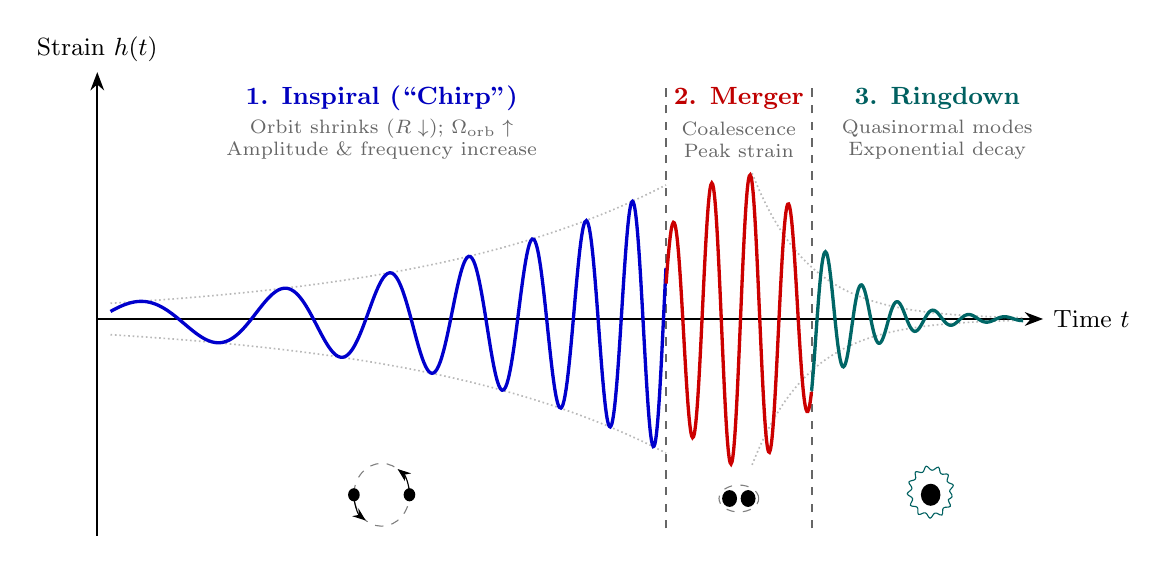
\begin{tikzpicture}[xscale=0.84, yscale=0.95, >=Stealth]
    % Axes
    \draw[->, thick] (0,0) -- (14.3,0) node[right, font=\small] {Time $t$};
    \draw[->, thick] (0,-2.9) -- (0,3.3) node[above, font=\small] {Strain $h(t)$};

    % Phase separator dashed lines
    \draw[dashed, gray!80!black, thick] (8.6,-2.8) -- (8.6,3.1);
    \draw[dashed, gray!80!black, thick] (10.8,-2.8) -- (10.8,3.1);

    % Phase headers placed cleanly above the peak waveform with plenty of horizontal separation
    \node[font=\bfseries\small, blue!75!black] at (4.3, 2.95) {1. Inspiral (``Chirp'')};
    \node[font=\scriptsize, align=center, text=gray!80!black] at (4.3, 2.40) {Orbit shrinks ($R \downarrow$); $\Omega_{\text{orb}} \uparrow$\\Amplitude \& frequency increase};

    \node[font=\bfseries\small, red!75!black] at (9.7, 2.95) {2. Merger};
    \node[font=\scriptsize, align=center, text=gray!80!black] at (9.7, 2.40) {Coalescence\\Peak strain};

    \node[font=\bfseries\small, teal!75!black] at (12.7, 2.95) {3. Ringdown};
    \node[font=\scriptsize, align=center, text=gray!80!black] at (12.7, 2.40) {Quasinormal modes\\Exponential decay};

    % Envelope curve (faint dashed)
    \draw[gray!55, densely dotted, semithick, domain=0.2:8.6, samples=100]
        plot (\x, {0.20 * exp(0.255*\x)});
    \draw[gray!55, densely dotted, semithick, domain=0.2:8.6, samples=100]
        plot (\x, {-0.20 * exp(0.255*\x)});
    \draw[gray!55, densely dotted, semithick, domain=9.9:14.0, samples=80]
        plot (\x, {1.95 * exp(-1.15*(\x-9.9))});
    \draw[gray!55, densely dotted, semithick, domain=9.9:14.0, samples=80]
        plot (\x, {-1.95 * exp(-1.15*(\x-9.9))});

    % Waveform: Inspiral + Merger + Ringdown
    % Inspiral: x from 0.2 to 8.6
    % At x = 8.6: phase = 2.5*8.6 + 0.036*(8.6)^3 = 21.5 + 22.898 = 44.398 rad
    % Amplitude at x = 8.6: 0.20 * exp(0.255*8.6) = 1.793
    \draw[blue!80!black, very thick, domain=0.2:8.6, samples=350, smooth]
        plot (\x, {0.20 * exp(0.255*\x) * sin((2.5*\x + 0.036*\x*\x*\x) r)});

    % Merger: x from 8.6 to 10.8, peaking around x = 9.7 with max amplitude 1.95
    \draw[red!80!black, very thick, domain=8.6:10.8, samples=160, smooth]
        plot (\x, {1.95 * exp(-0.42*(\x-9.7)*(\x-9.7)) * sin((44.398 + 10.8*(\x-8.6)) r)});

    % Ringdown: x from 10.8 to 14.0, damped sinusoid at high constant frequency
    % At x = 10.8: amplitude = 1.95 * exp(-0.42*1.21) = 1.173, phase = 44.398 + 10.8*2.2 = 68.158 rad
    \draw[teal!80!black, very thick, domain=10.8:14.0, samples=200, smooth]
        plot (\x, {1.173 * exp(-1.25*(\x-10.8)) * sin((68.158 + 11.6*(\x-10.8)) r)});

    % Schematic diagrams of the binary below the waveform
    % Inspiral binary
    \draw[gray, dashed] (4.3,-2.35) circle (0.42);
    \fill[black] (4.72,-2.35) circle (2.5pt);
    \fill[black] (3.88,-2.35) circle (2.5pt);
    \draw[->, thin] (4.72,-2.35) arc (0:55:0.42);
    \draw[->, thin] (3.88,-2.35) arc (180:235:0.42);

    % Merger binary (touching/plunging)
    \fill[black] (9.56,-2.40) circle (3.2pt);
    \fill[black] (9.84,-2.40) circle (3.2pt);
    \draw[gray, dashed] (9.7,-2.40) ellipse (0.30 and 0.18);

    % Ringdown single black hole settling
    \fill[black] (12.6,-2.35) circle (4.2pt);
    \draw[teal!75!black, decorate, decoration={snake, amplitude=0.8pt, segment length=4pt}] (12.6,-2.35) circle (0.32);
\end{tikzpicture}
\end{center}
\end{enumerate}

\end{document}
